\documentclass{article}
\usepackage{tikz-er2}
\usepackage[simplified]{pgf-umlcd}
\usepackage[output=answers]{mcexam}

\usetikzlibrary{er}

\begin{document}

\tikzstyle{every entity} = [fill=blue!20]
\tikzstyle{every attribute} = [fill=yellow!20]
\tikzstyle{every relationship} = [fill=red!20]
\tikzstyle{every edge} = [link]

\begin{tikzpicture}[node distance=6em]
 \node[entity] (person) {Person};
 \node[attribute] (pid) [left of=person] {\key{ID}} edge (person);
 \node[attribute] (name) [above left of=person] {Name} edge (person);
 \node[derived attribute] (age) [above of=person] {Age} edge (person);
 \node[relationship] (uses) [right of=person] {Uses} edge (person);
 \node[entity] (tool) [right of=uses] {Tool} edge (uses);
\end{tikzpicture}

Aqui poderia estar escrito um texto qualquer para mostrar o quanto eu estou me importando com as coisas...\footnote{Isso é apenas um teste}

\begin{tikzpicture}[node  distance=6em]
 \node[entity] (person) {Person};
 \node[attribute] (pid) [left of=person] {\key{ID}} edge (person);
 \node[attribute] (name) [above  left of=person] {Name} edge (person);
 \node[multi  attribute] (phone) [above  of=person] {Phone} edge (person);
 \node[attribute] (address) [above  right  of=person] {Address} edge (person);
 \node[attribute] (street) [above  right  of=address] {Street} edge (address);
 \node[attribute] (city) [right  of=address] {City} edge (address);
 \node[derived  attribute] (age) [right  of=person] {Age} edge (person);
 \node[relationship] (uses) [below  of=person] {Uses} edge (person);
 \node[entity] (tool) [below  of=uses] {Tool} edge[total] (uses);
 \node[attribute] (tid) [left of=tool] {\key{ID}} edge (tool);
 \node[attribute] (tname)[right  of =tool] {Name} edge (tool);
\end{tikzpicture}

Ta queu

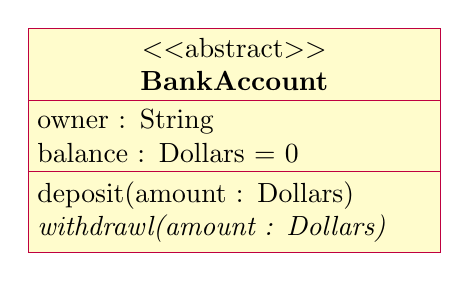
\begin{tikzpicture}
  \begin{abstractclass}[text width=5cm]{ BankAccount}{0 ,0}
    \attribute{owner : String}
    \attribute{balance : Dollars = 0}
    \operation{deposit(amount : Dollars)}
    \operation [0]{ withdrawl(amount : Dollars)}
  \end{abstractclass}
\end{tikzpicture}

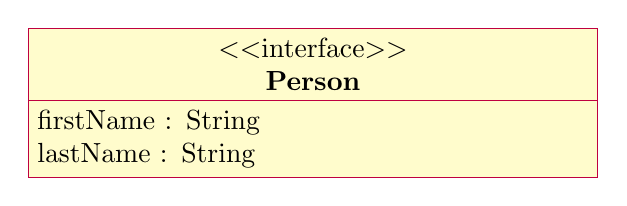
\begin{tikzpicture}
  \begin{interface}[text width=7cm]{ Person }{0,0}
    \attribute{firstName : String}
    \attribute{lastName : String}
  \end{interface}
\end{tikzpicture}

Ta queu

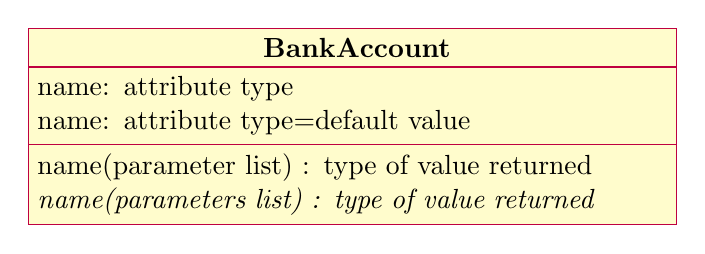
\begin{tikzpicture}
  \begin{class}[text width=8cm]{ BankAccount }{0,0}
    \attribute{name: attribute  type}
    \attribute{name: attribute  type=default value}
    \operation{name(parameter  list) : type of value returned}
    %  virtual  operation
    \operation [0]{ name(parameters  list) : type of value  returned}
  \end{class}
\end{tikzpicture}

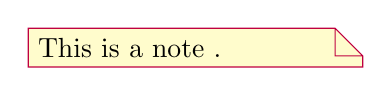
\begin{tikzpicture}
  \umlnote (note) {This is a note .};
\end{tikzpicture}

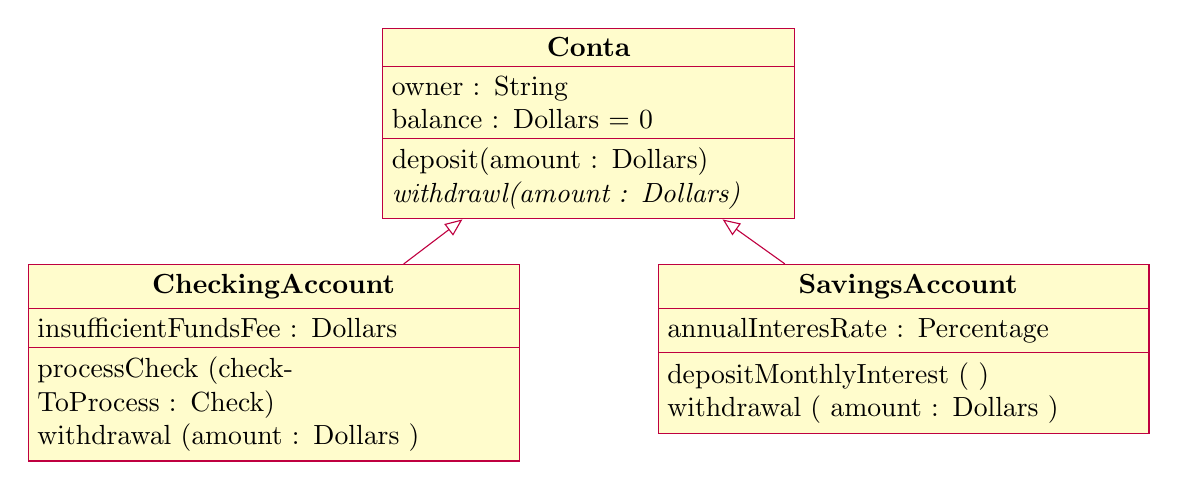
\begin{tikzpicture}
 \begin{class}[text width=5cm]{Conta}{0,0}
   \attribute{owner : String}
   \attribute{balance : Dollars = 0}
   \operation{deposit(amount : Dollars)}
   \operation [0]{withdrawl(amount : Dollars)}
 \end{class}
  
 \begin{class}[text  width=6cm]{CheckingAccount}{-4,-3}
   \inherit{Conta}
   \attribute{insufficientFundsFee : Dollars}
   \operation{processCheck (checkToProcess : Check)}
   \operation{withdrawal (amount : Dollars )}
 \end{class}
 
 \begin{class}[text  width=6cm]{ SavingsAccount }{4,-3}
   \inherit{Conta}
   \attribute{annualInteresRate : Percentage}
   \operation{depositMonthlyInterest ( )}
   \operation{withdrawal ( amount : Dollars )}
 \end{class}
 
\end{tikzpicture}


\begin{mcquestions}
\question How much is $2+2$?
\begin{mcanswerslist}
\answer two
\answer[correct] four
\answer five
\end{mcanswerslist}
\question How much is $5-3$?
\begin{mcanswerslist}
\answer 1
\answer[correct] 2
\answer 3
\end{mcanswerslist}
\end{mcquestions}
\end{document}

